\begin{figure}
    \begin{center}
        \subfloat[From experiment 2\textunderscore 1691621262 at checkpoint 5000 ]{
            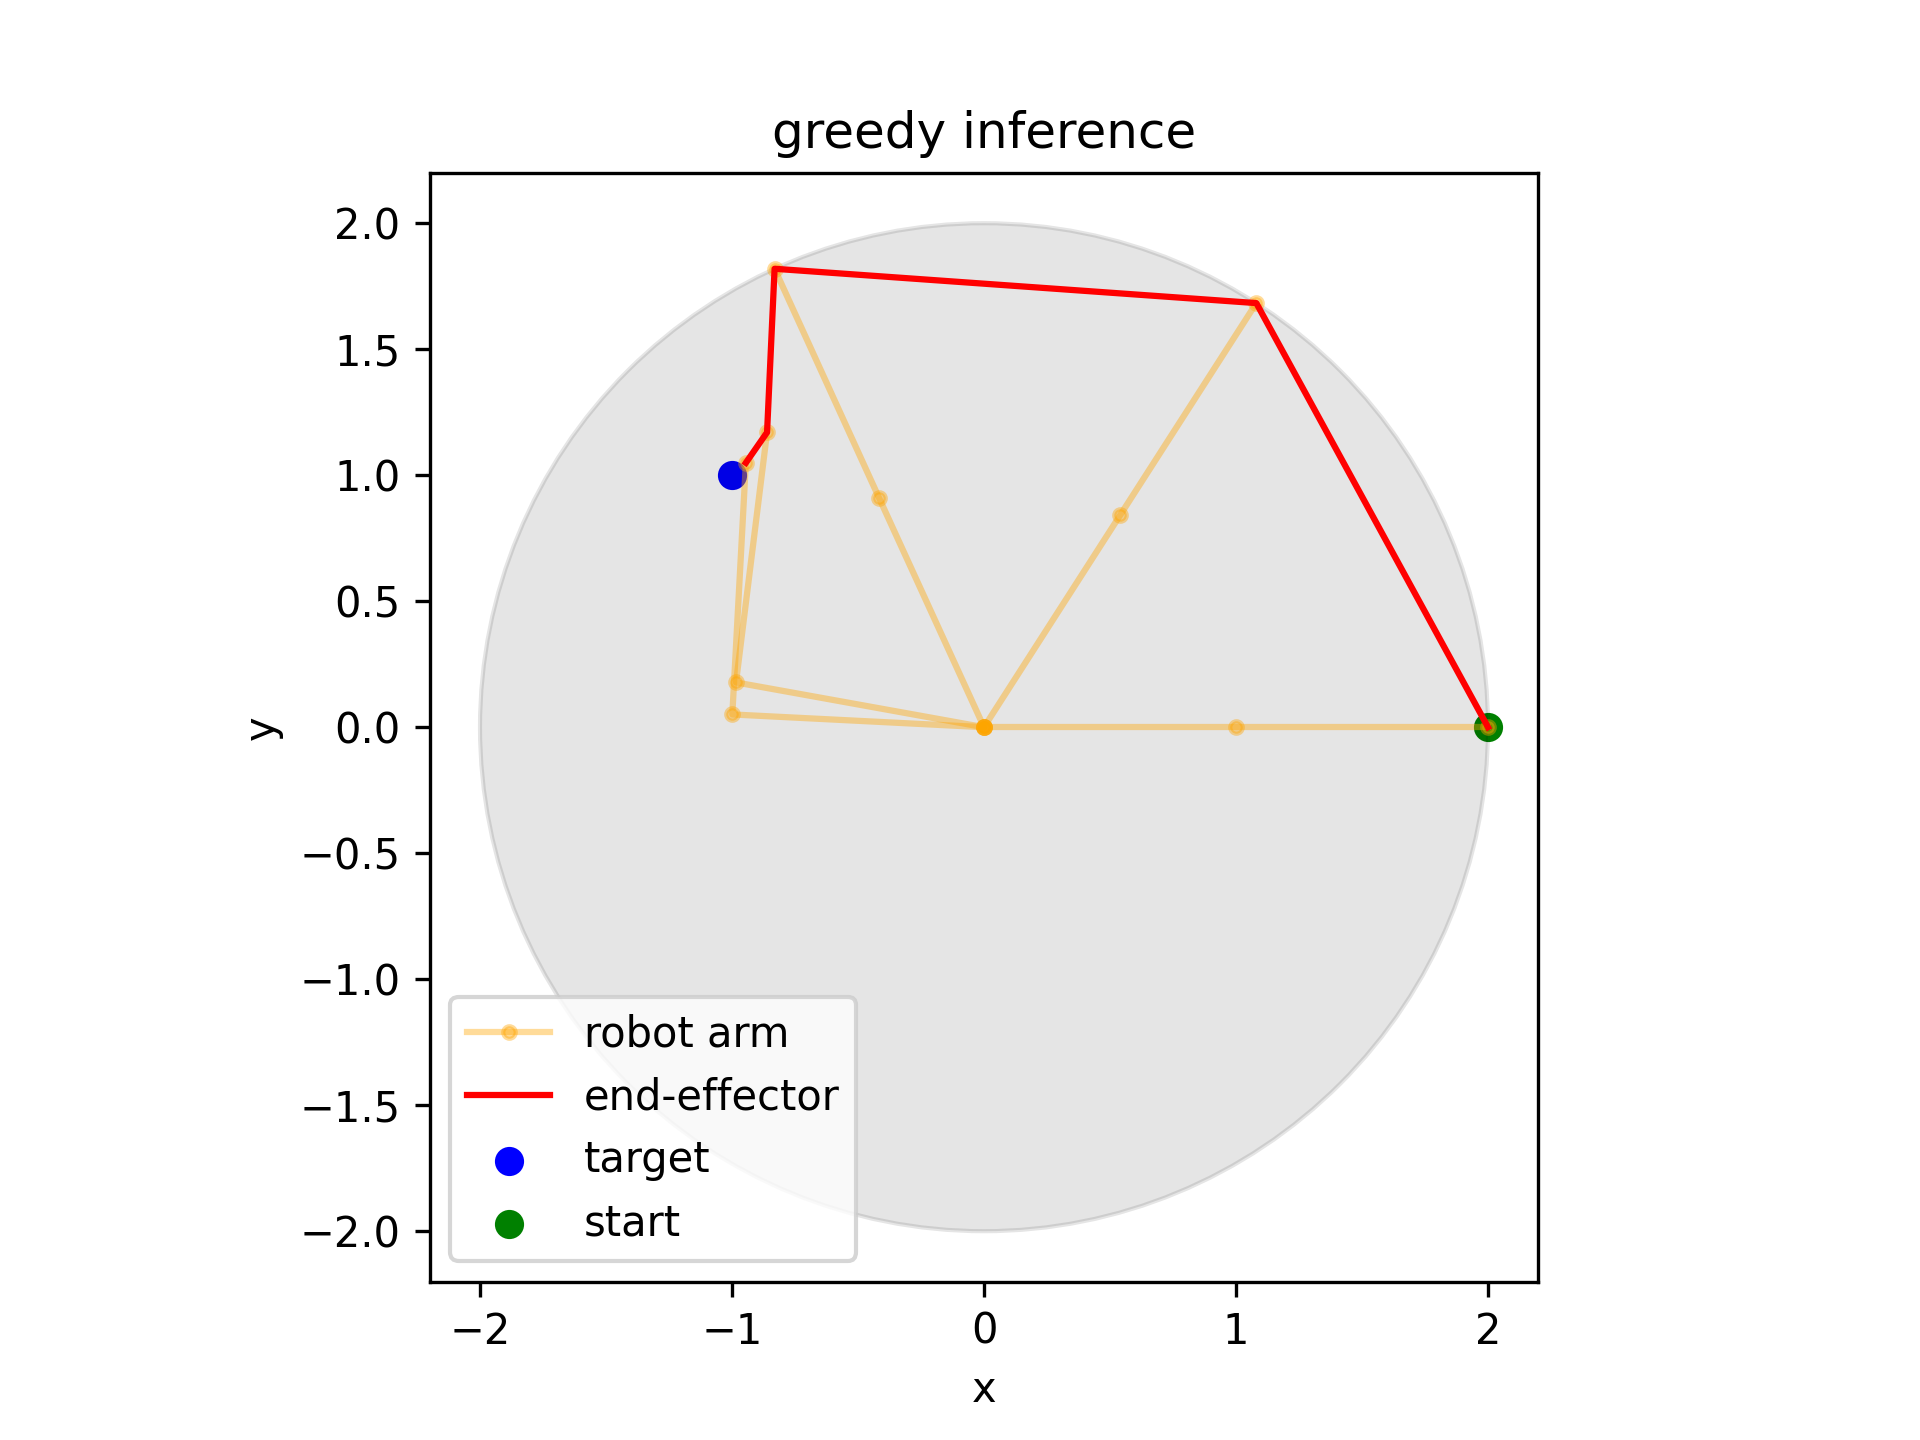
\includegraphics[width=0.46 \linewidth]{figures/experiments/greedy_inference_baseline_2_1691621262_5000.png}
            \label{fig:SAC_baseline_inference_trajectory/greedy_2}
            }
        \hfill
        \subfloat[From experiment 5\textunderscore 1691624939 at checkpoint 5000. To make things more clear only every 5th robot arm is drawn]{
            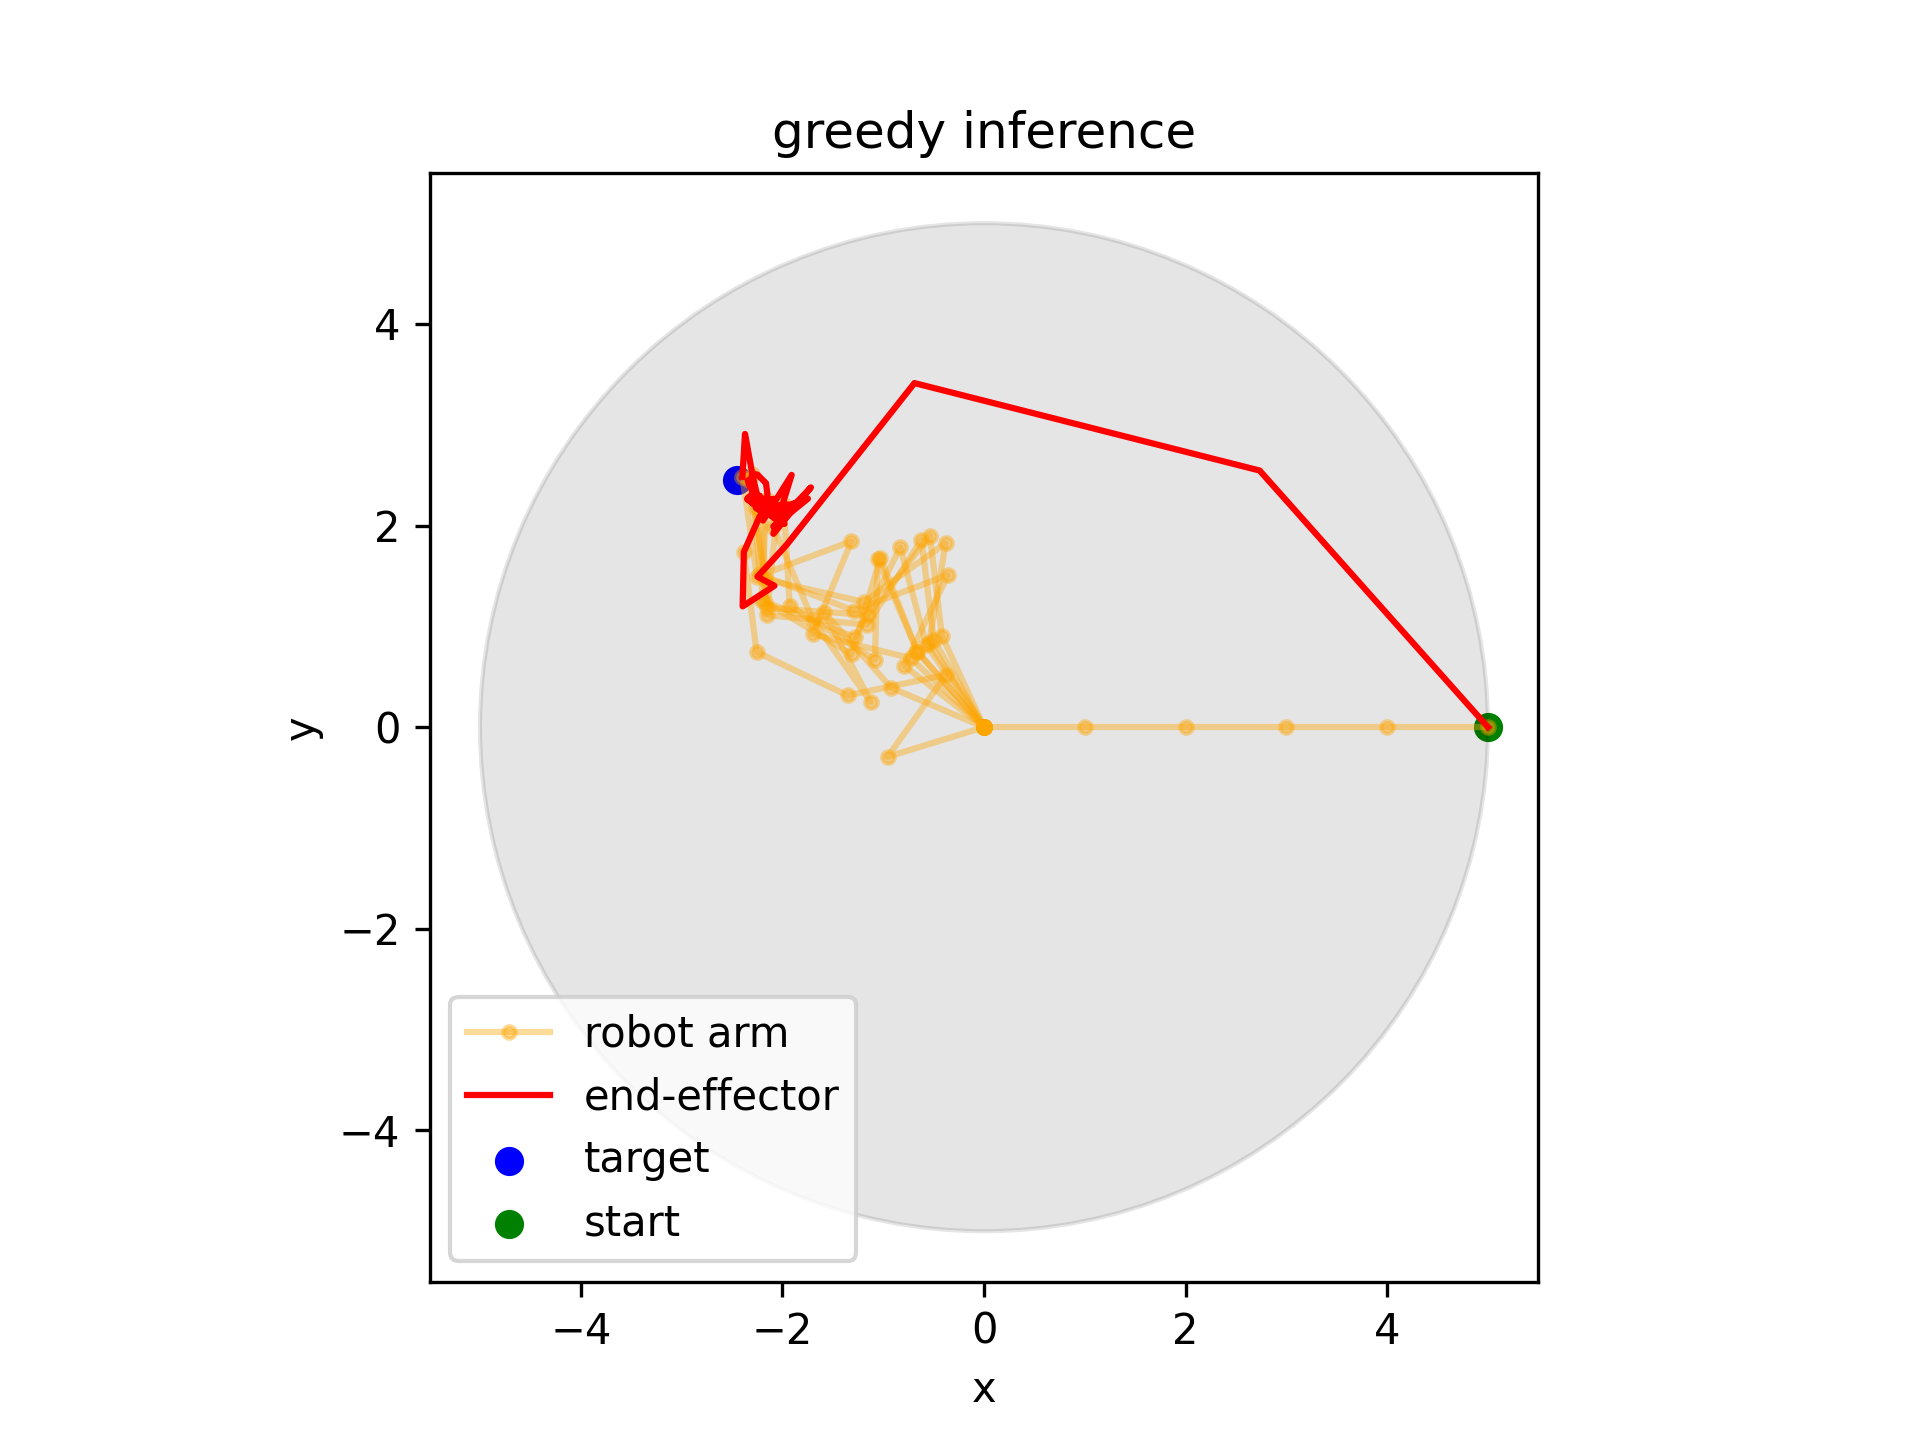
\includegraphics[width=0.46 \linewidth]{figures/experiments/greedy_inference_baseline_5_1691624939_5000.png}
            \label{fig:SAC_baseline_inference_trajectory/greedy_5}
            }\\
        \subfloat[From experiment XXX at checkpoint 5000.To make things more clear only every 5th robot arm is drawn]{
            
\includegraphics[width=0.46 \linewidth]{figures/place_holder.png}
            \label{fig:SAC_baseline_inference_trajectory/greedy_10}
            }
        \hfill
        \subfloat[From experiment 15\textunderscore 1691619106 at checkpoint 5000. To make things more clear only every 40th robot arm is drawn]{
            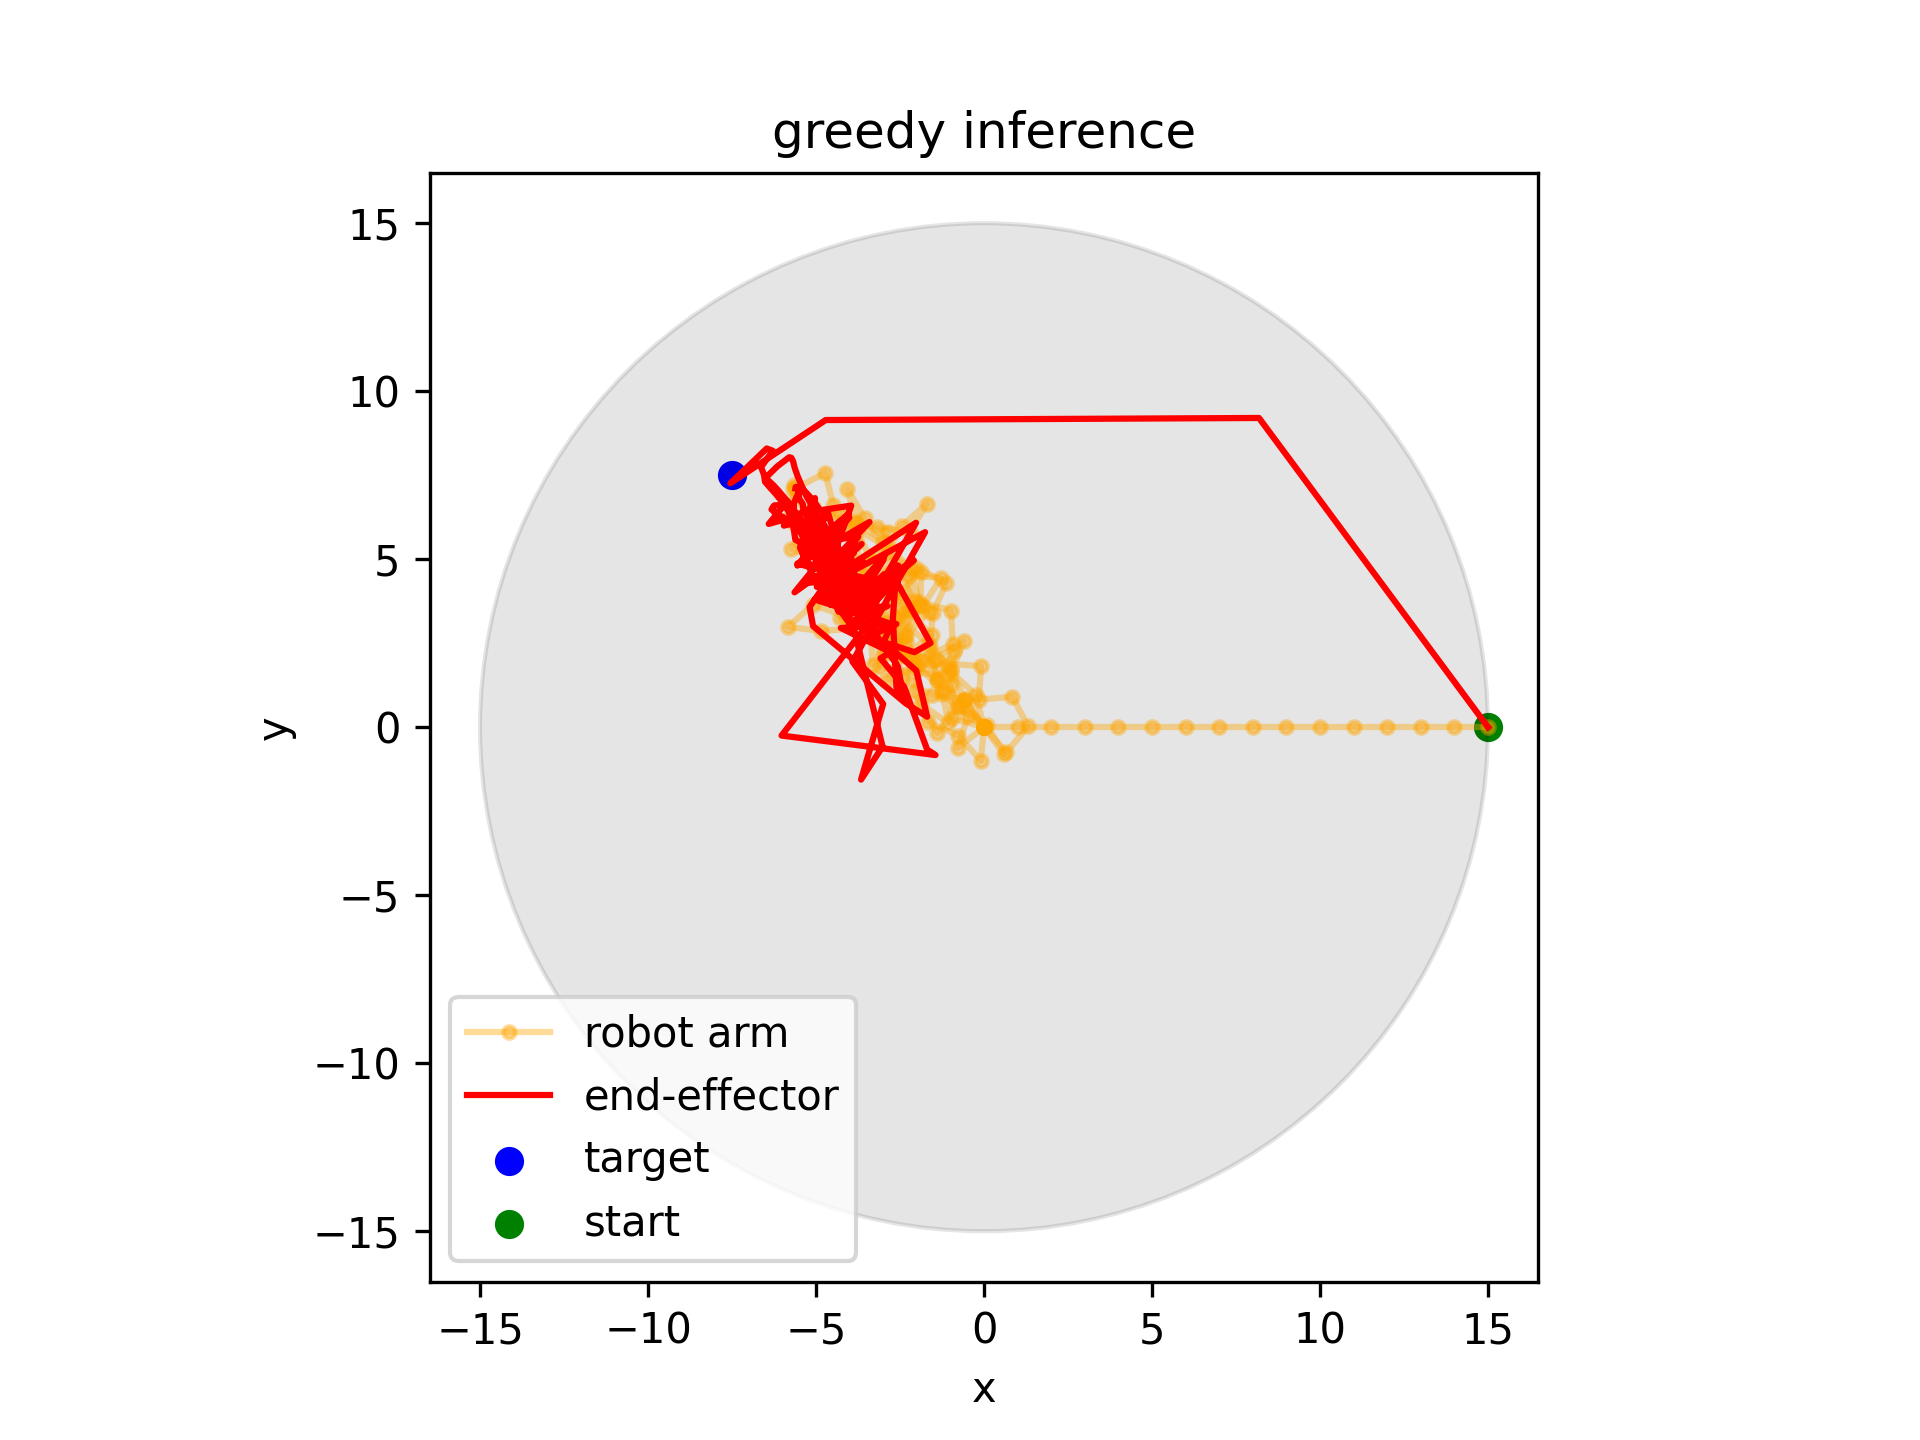
\includegraphics[width=0.46 \linewidth]{figures/experiments/greedy_inference_baseline_15_1691619106_5000.png}
            \label{fig:SAC_baseline_inference_trajectory/greedy_15}
            }
        \\
        \subfloat[From experiment 20\textunderscore 1691619159 at checkpoint 5000. To make things more clear only every 40th robot arm is drawn]{
            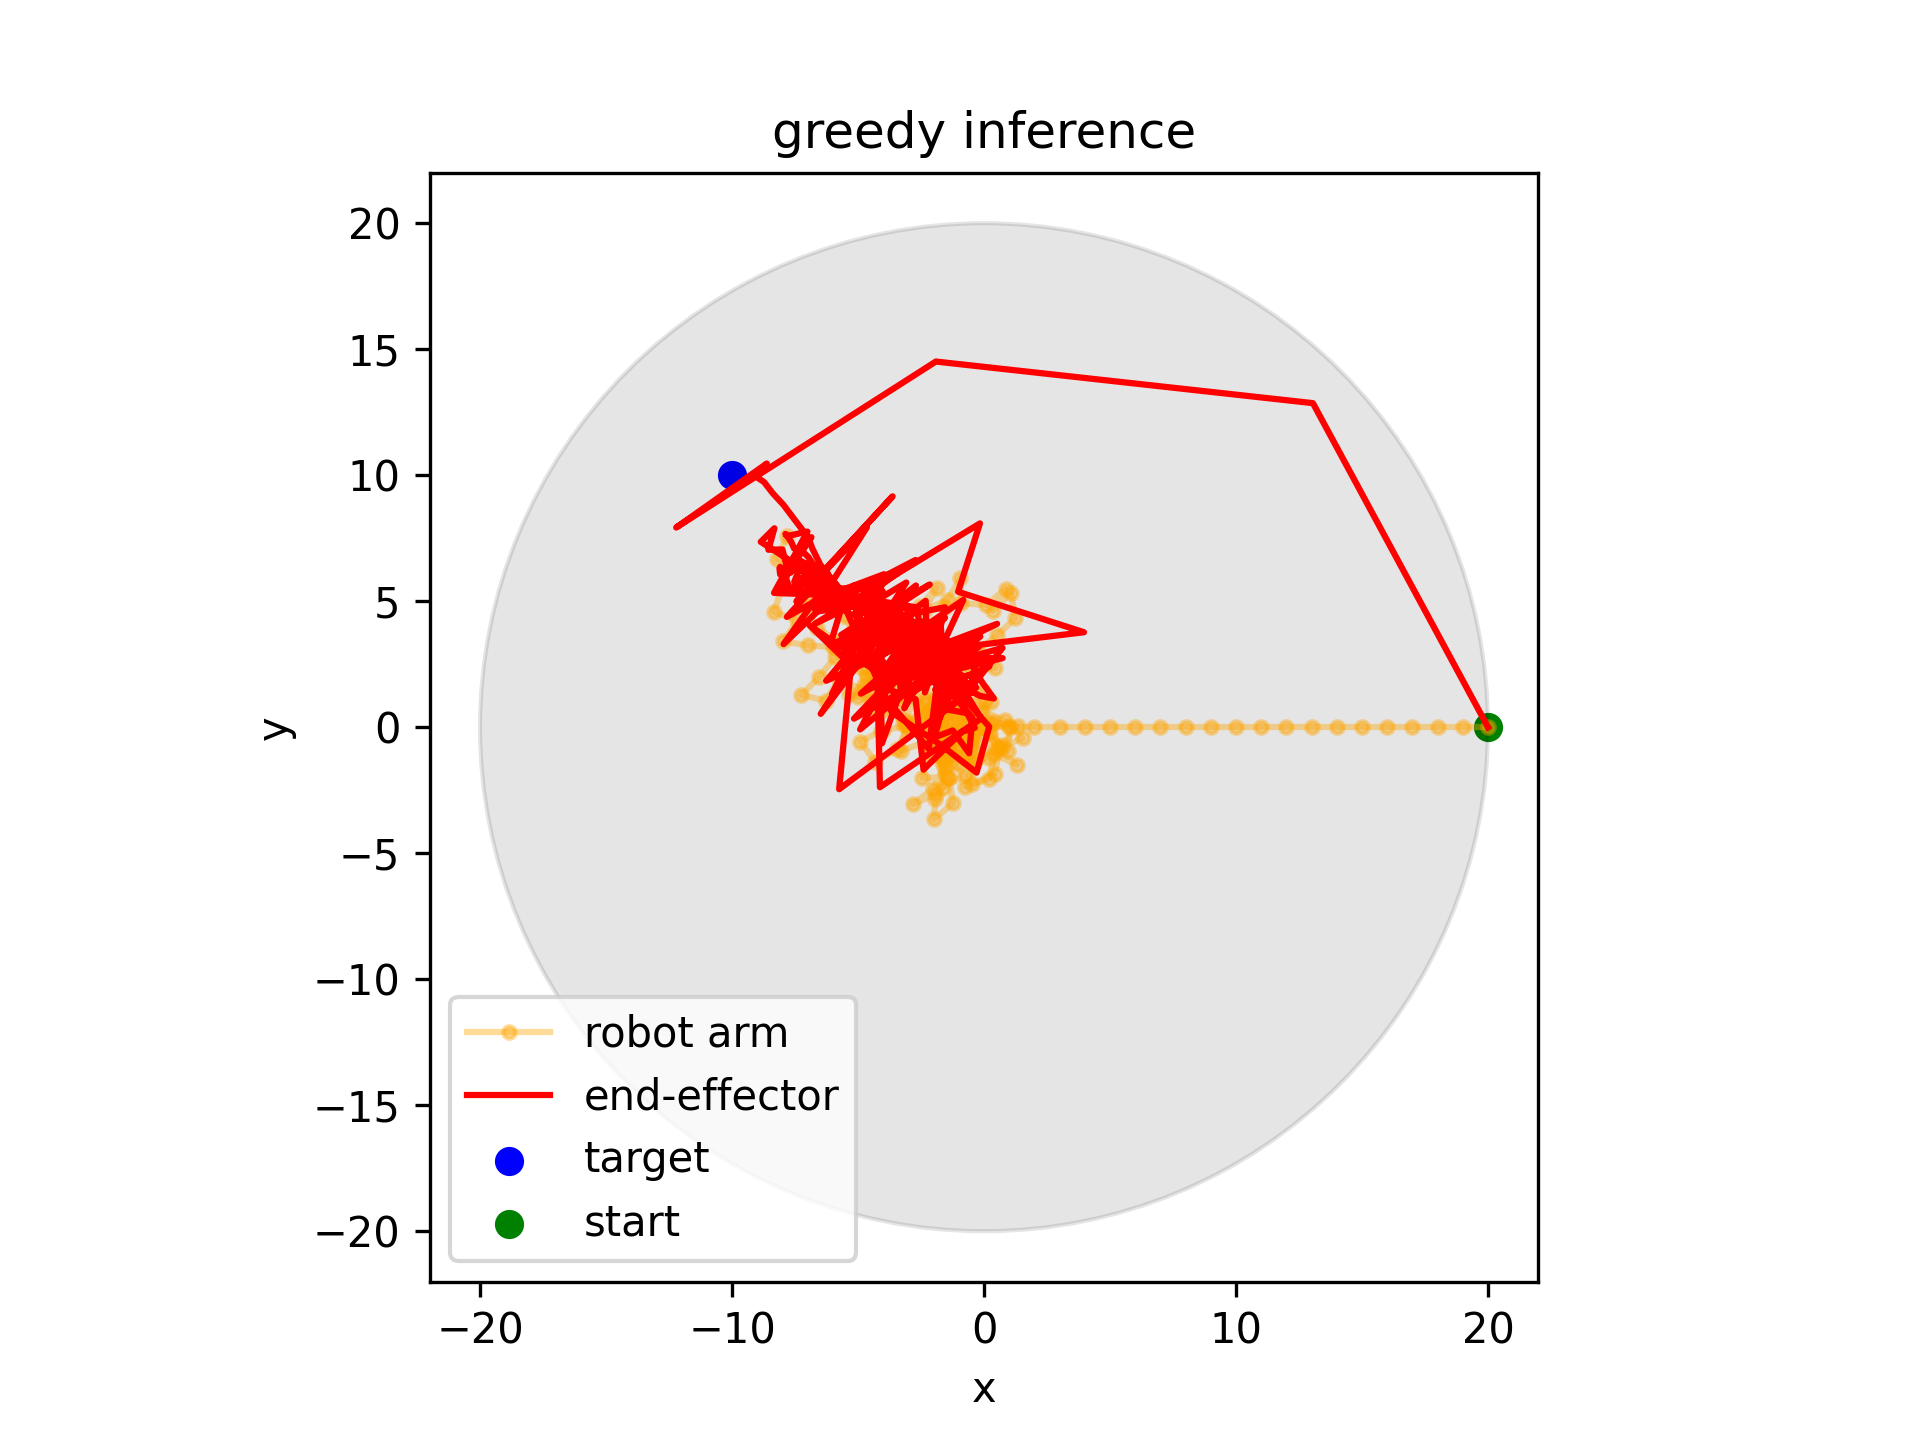
\includegraphics[width=0.46 \linewidth]{figures/experiments/greedy_inference_baseline_20_1691619159_5000.png}
            \label{fig:SAC_baseline_inference_trajectory/greedy_20}
            }
    \end{center}
    \caption[SAC baseline inference]{SAC inference. The trajectory is plotted in red. robot arms are drawn in yellow with the little dots as positions of each joint. Target position and start position are scattered in blue and green. The space an end-effector is able to reach is plotted in grey.}
    \label{fig:SAC_baseline_inference_trajectory}
\end{figure}

\begin{figure}
    \begin{center}
        \subfloat[Distance to target policy from experiment 2\textunderscore 1691621262 at checkpoint 5000 ]{
        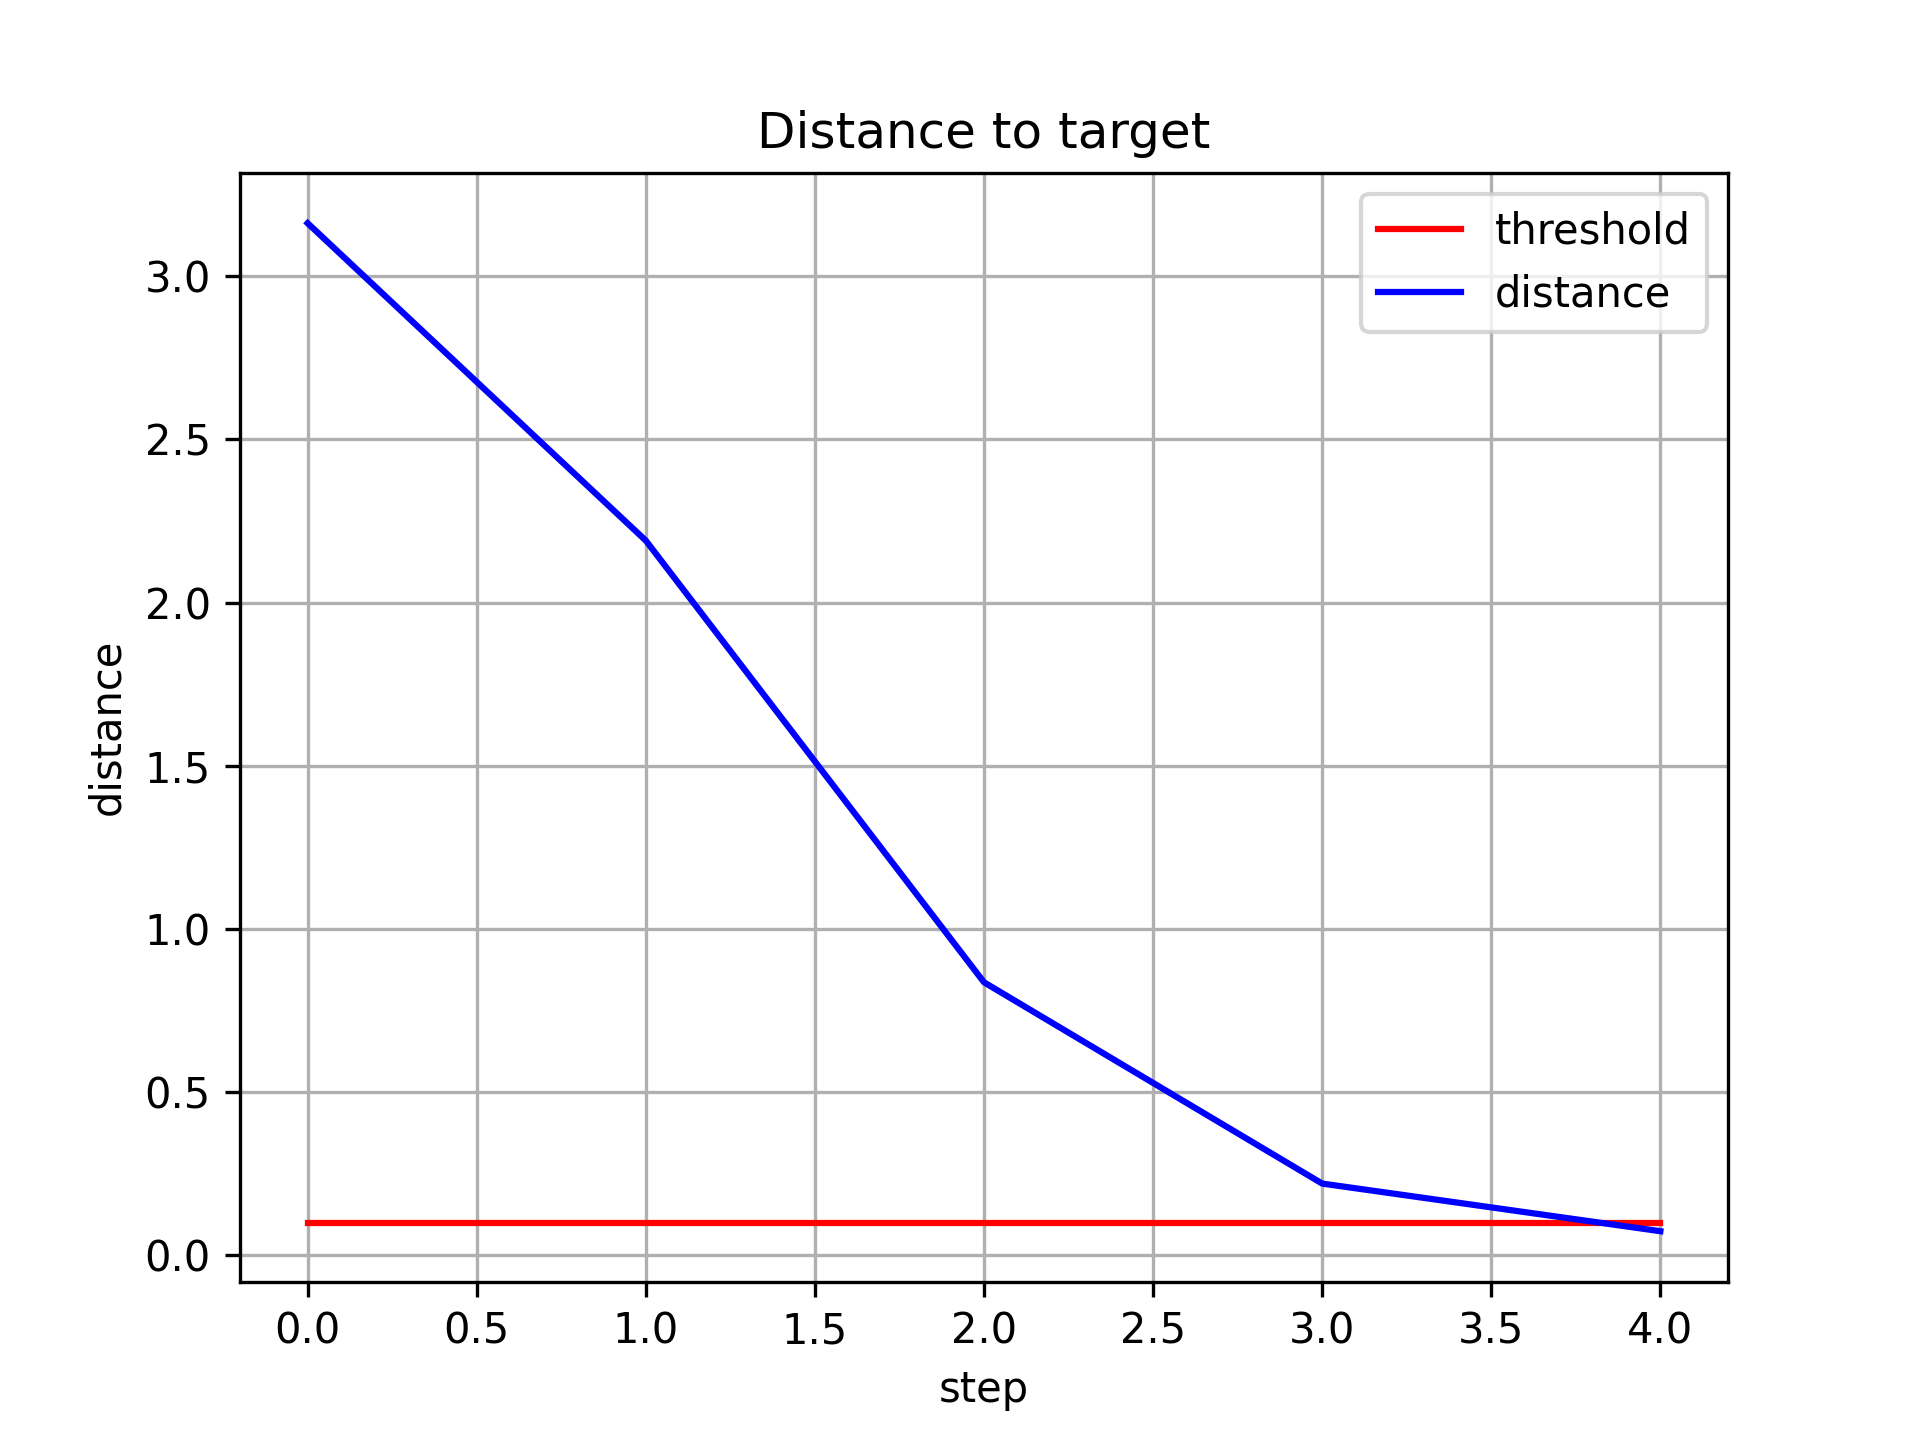
\includegraphics[width=0.46 \linewidth]{figures/experiments/Distance_to_target_baseline_2_1691621262_5000.png}
            \label{fig:SAC_baseline_inference/distance_2}
            }
        \hfill
        \subfloat[Distance to target policy from experiment 5\textunderscore 1691624939 at checkpoint 5000 ]{
        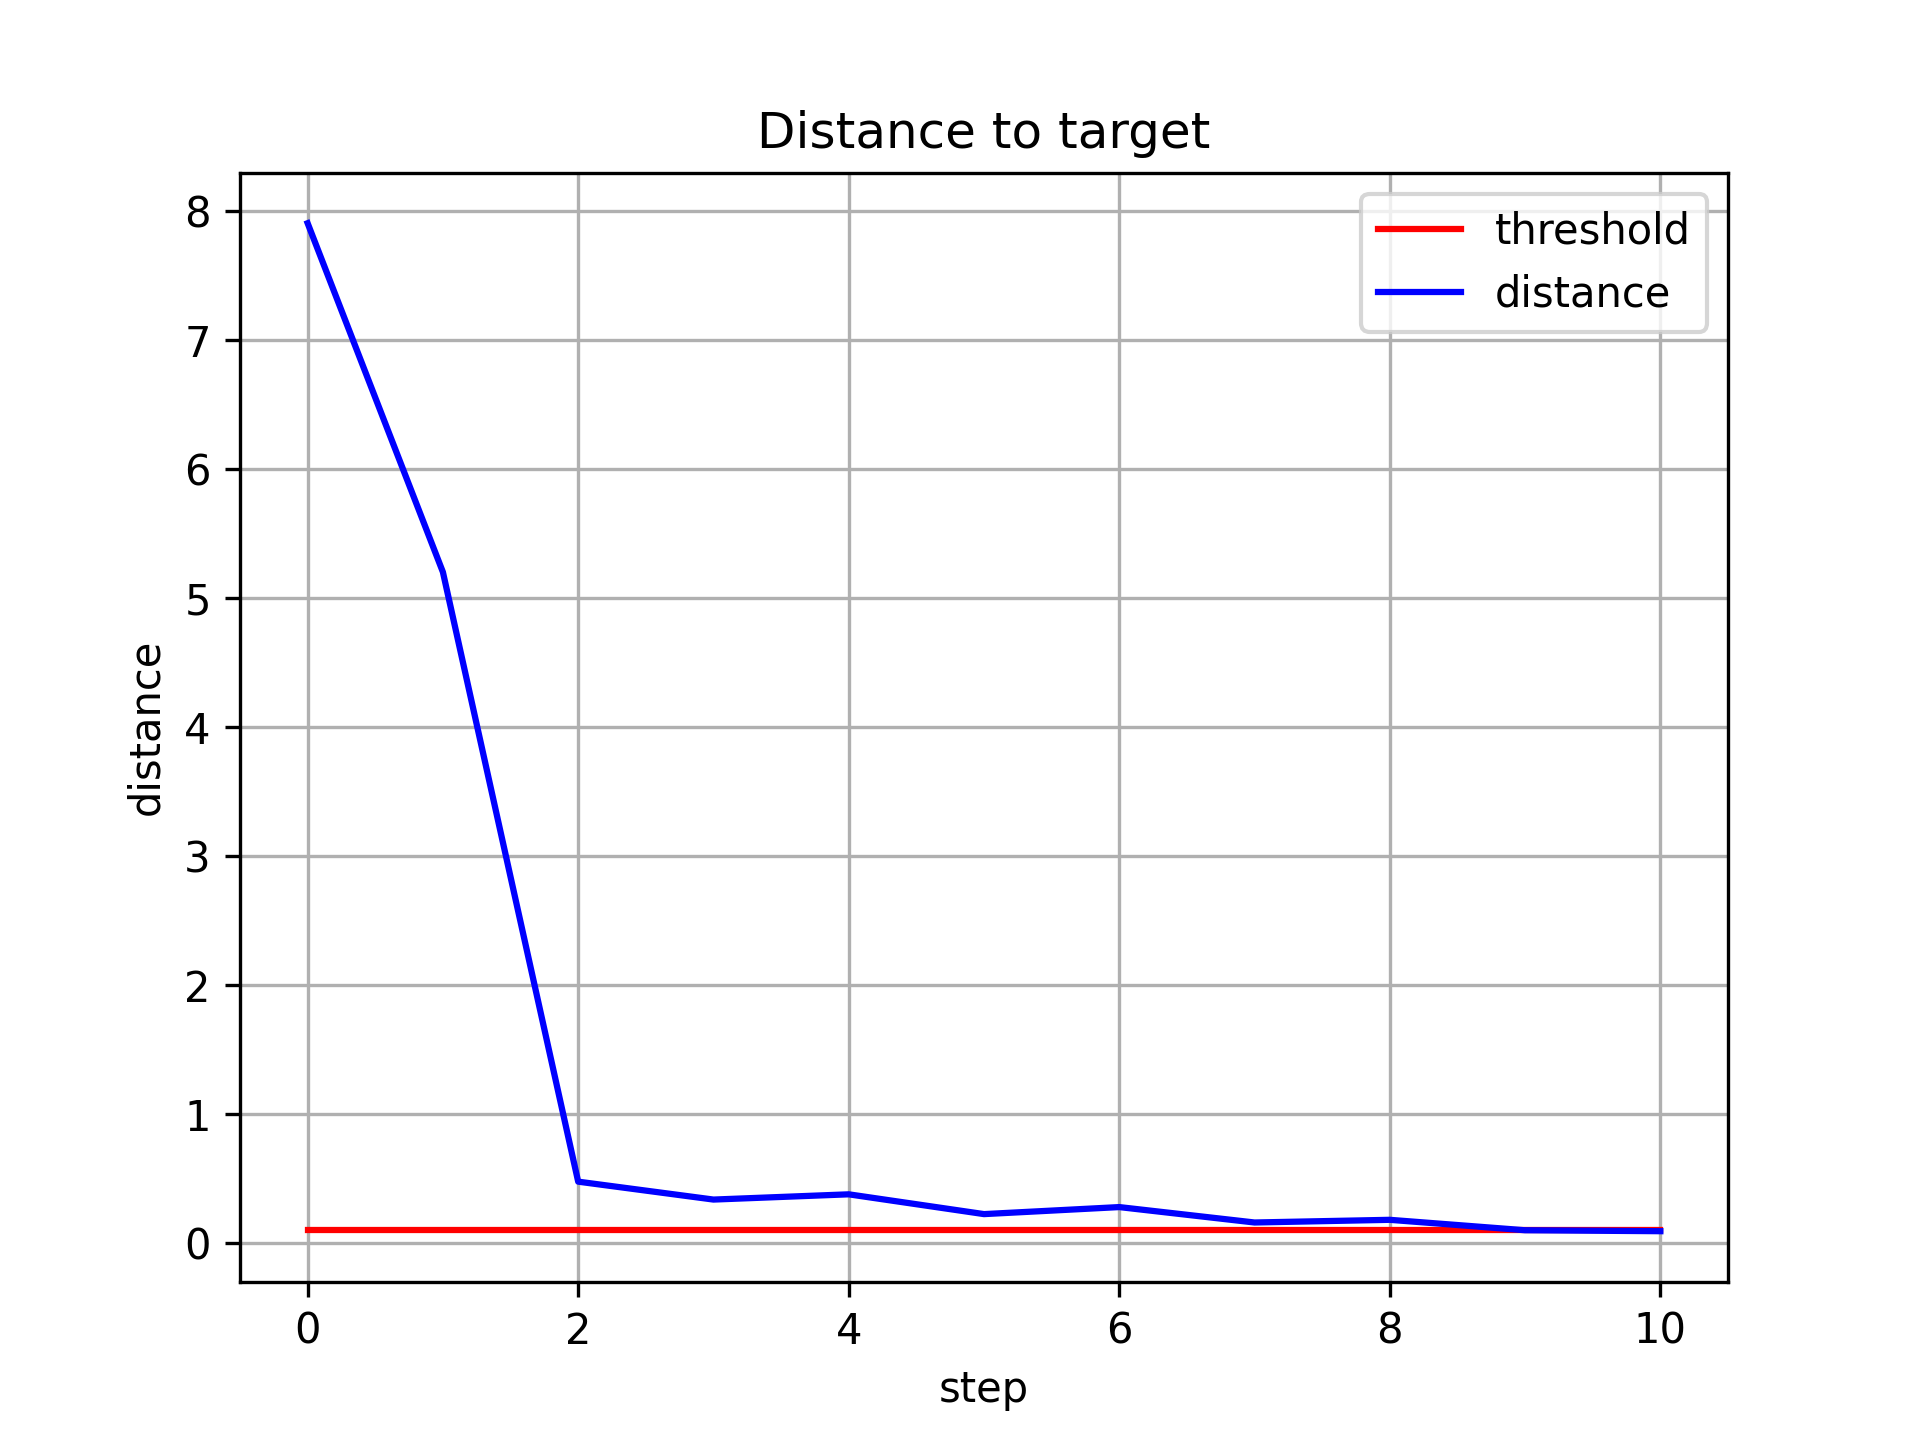
\includegraphics[width=0.46 \linewidth]{figures/experiments/Distance_to_target_baseline_5_1691624939_5000.png}
            \label{fig:SAC_baseline_inference/distance_5}
            } \\
        \subfloat[Distance to target policy from experiment XXX at checkpoint 5000 ]{
        
\includegraphics[width=0.46 \linewidth]{figures/place_holder.png}
            \label{fig:SAC_baseline_inference/distance_10}
            }
        \hfill
        \subfloat[Distance to target policy from experiment 15\textunderscore 1691619106 at checkpoint 5000 ]{
        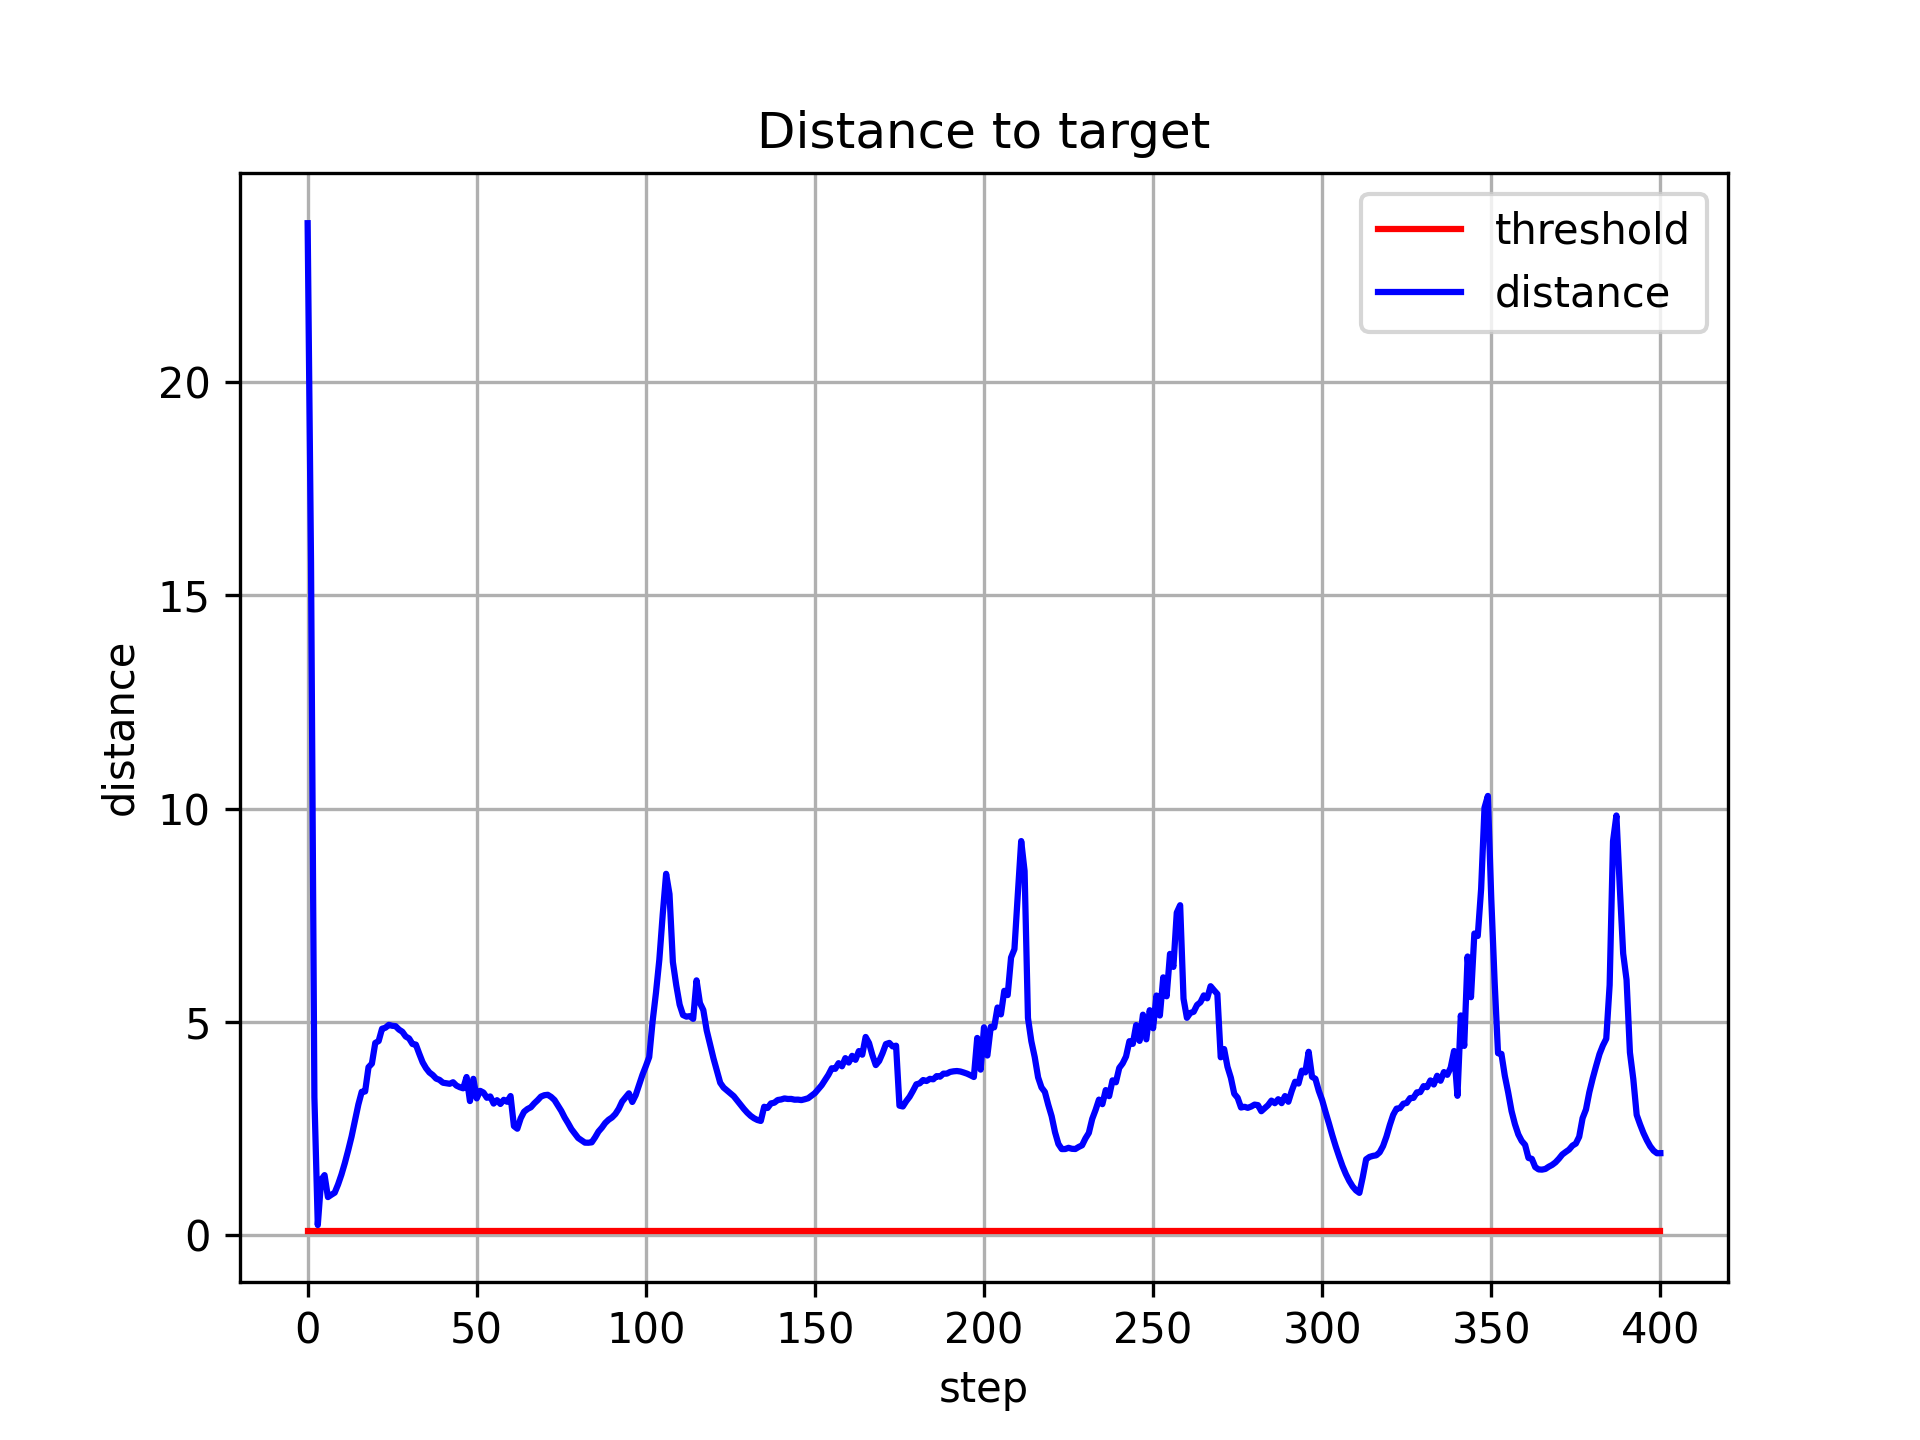
\includegraphics[width=0.46 \linewidth]{figures/experiments/Distance_to_target_baseline_15_1691619106_5000.png}
            \label{fig:SAC_baseline_inference/distance_15}
            } \\
        \subfloat[Distance to target policy from experiment 20\textunderscore 1691619159 at checkpoint 5000 ]{
        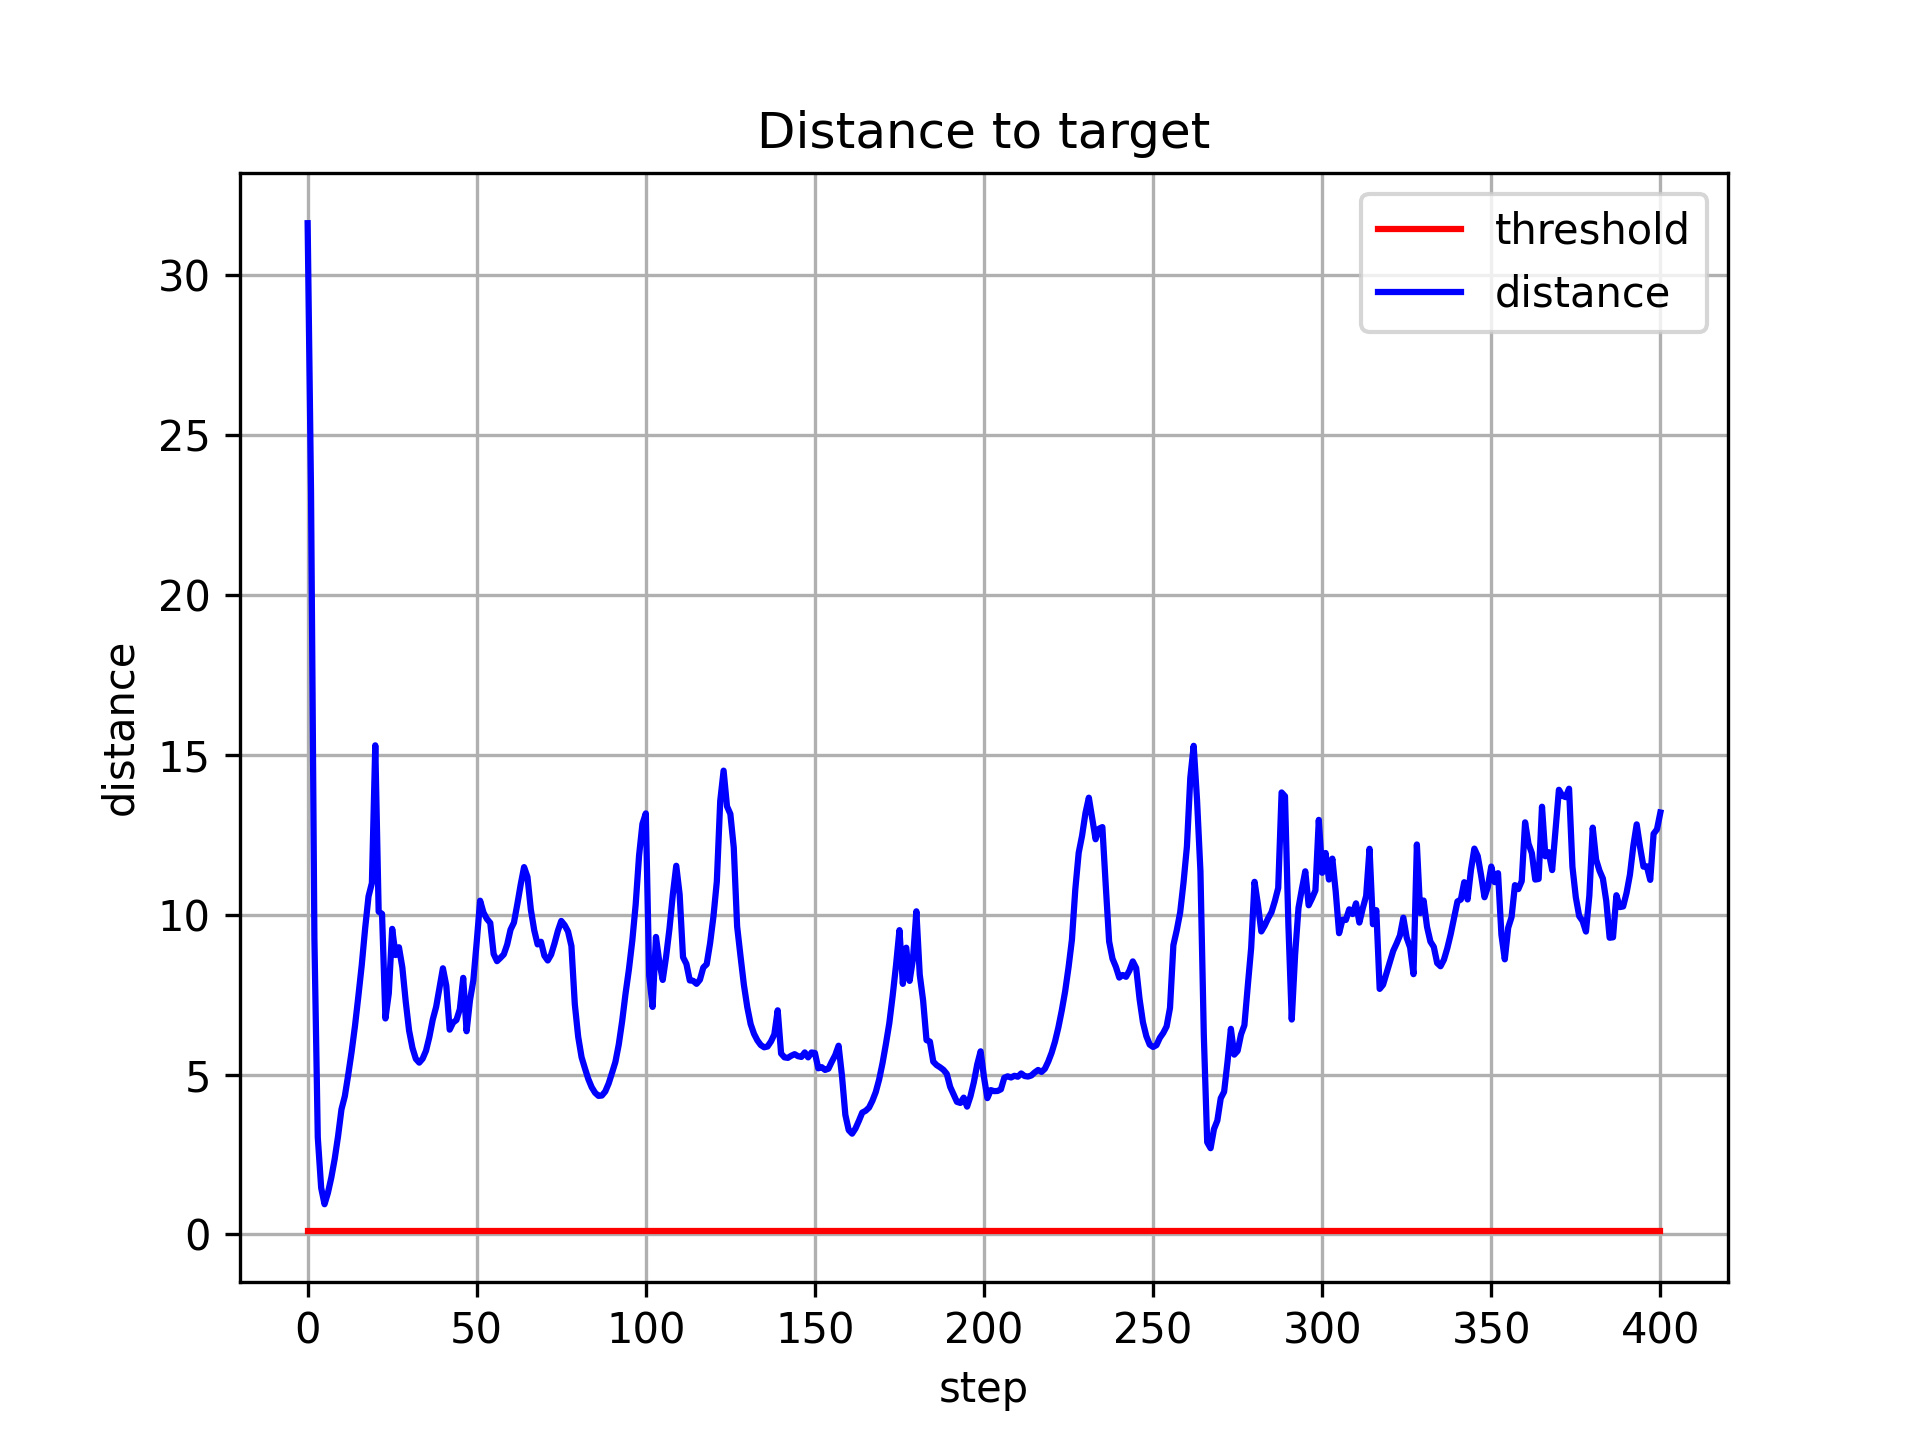
\includegraphics[width=0.46 \linewidth]{figures/experiments/Distance_to_target_baseline_20_1691619159_5000.png}
            \label{fig:SAC_baseline_inference/distance_20}
            }
    \end{center}
    \caption[SAC baseline inference]{Distance to target for each action outcome. The target is consistent at $[-0.5, 0.5] \cdot n\text{\textunderscore} joints$. The threshold of 0.1 at which an episode is concluded successfully is drawn in red.} 
    \label{fig:SAC_baseline_inference_distance}
\end{figure}